\section{Wahrscheinlichkeitsverteilung}
\kopfrechts{Wahrscheinlichkeitsverteilung}
\begin{figure}
\begin{center}
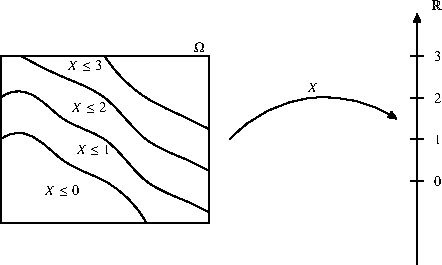
\includegraphics[width=0.7\hsize]{images/verteilungsfunktion-1}
\end{center}
\caption{Übergang von $\Omega$ zu Werten
der Zufallsvariablen $X$.
\label{bilduebergangzurverteilungsfunktion}}
\end{figure}
In diesem Abschnitt reduzieren wir die Information in einer Zufallsvariable
$X\colon\Omega\to\mathbb R$ auf einfache Funktionen einer reellen Veränderlichen.
Wir werden feststellen, dass die Verteilungsfunktion sowohl stetige wie auch
diskrete Zufallsvariablen gleichermassen beschreiben kann, dass wir
aber verschiedene analytische Methoden verwenden müssen, um daraus
Erwartungswerte zu berechnen.

\subsection{Verteilungsfunktion}
\index{Verteilungsfunktion}
\begin{figure}
\begin{center}
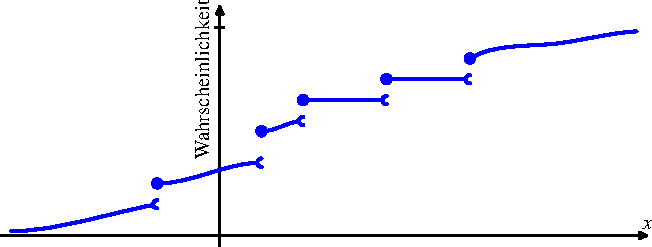
\includegraphics{images/verteilungsfunktion-2}
\end{center}
\caption{Die Verteilungsfunktion $F$ einer Zufallsvariablen $X$,
$F(x)=P(X\le x)$, zeigt die Wahrscheinlichkeit dafür, dass $X$ den Wert $x$ nicht
überschreitet.
\label{bildverteilungsfunktion}}
\end{figure}
Aus einem Wahrscheinlichkeitsmass $P$ auf $\Omega$ kann man mit Hilfe
von $X$ auch ein Wahrscheinlichkeitsmass auf $\mathbb{R}$ bilden.
Für die
Wahrscheinlichkeit für das Intervall $[a,b]\subset\mathbb{R}$ setzt
man einfach
\[
P((a,b])=P(a< X\le b).
%=P(X^{-1}((a,b])),
\]
Das letzte $P$ ist dabei als Wahrscheinlichkeit eines Ereignisses $\Omega$
bereits bekannt.
Noch etwas handlicher ist die folgende Definition.

\begin{definition}
\label{verteilung:definition:verteilungsfunktion}
Die Funktion $F\colon\mathbb{R}\to\mathbb{R}:x\mapsto P(X\le x)$
heisst Verteilungsfunktion von $P$.
\end{definition}
Die folgenden Eigenschaften folgen unmittelbar aus dieser Definition:
\begin{enumerate}
\item Der Wertebereich von $F(x)$ ist im Intervall $[0,1]$ enthalten.
\item Die Funktion $F(x)$ ist monoton wachsend:
Da $\{ X \le a\} \subset \{X\le b\}$ falls $a\le b$ folgt
$F(a)=P(X\le a)\le P(X\le b)=F(b)$.
\item
Die Wahrscheinlichkeit des unmöglichen Ereignisses ist $0$, also
ist
\[
\lim_{x\to-\infty}F(x)=0.
\]
\item
Die Wahrscheinlichkeit des sicheren Ereignisses ist $1$, also gilt.
\[
\lim_{x\to\infty}F(x)=1.
\]
\end{enumerate}

Die Verteilungsfunktion $F$ beinhaltet alle Information, um $P$ zu
rekonstruieren.
Man kann mit ihrer Hilfe auch die Wahrscheinlichkeit
abgeschlossener Intervalle oder offener Intervalle berechnen:
\begin{satz} Sei $F$ die Verteilungsfunktion der Zufallsvariablen $X$,
dann gilt
\begin{align*}
P((a,b])&=F(b)-F(a)\\
P([a,b])&=\lim_{\xi\to a-} P((\xi,b])=F(b)-\lim_{\xi\to a-}F(\xi)\\
P((a,b))&=\lim_{\xi\to b-} P((a,\xi])=\lim_{\xi\to b-}F(\xi)-F(a)\\
P([a,b))&=\lim_{\eta\to b-}\lim_{\xi\to a-} P((\xi,\eta])=\lim_{\eta\to b-}F(\eta)-\lim_{\xi\to a-}F(\xi).
\end{align*}
\end{satz}
\begin{proof}[Beweis]Durch Nachrechnen unmittelbar aus den Definitionen.
\end{proof}

\subsection{Sprungstellen und diskrete Werte einer Zufallsvariable}
Als Spezialfall erhält man aus $F(x)$ auch die Wahrscheinlichkeit für einen
einzelnen Wert
\[
P(a)=P([a,a])=F(a)-\lim_{\xi\to a-}F(\xi).
\]
Solange die Funktion $F$ stetig ist, wird diese Wahrscheinlichkeit
verschwinden.
Andernfalls hat die Verteilungsfunktion am Punkt $a$ eine
Sprungstelle, und die Wahrscheinlichkeit, dass der Wert $a$ eintritt,
ist gerade die Sprunghöhe.

Man kann zeigen, dass eine monotone Funktion nur abzählbar viele Sprungstellen
hat.
Es gibt also eine Folge $(a_k)_{k\in\mathbb{N}}$, welche alle
Sprungstellen enthält.
Diese Werte zeichnen sich dadurch aus, dass ihre
Wahrscheinlichkeit nicht $0$ ist und der Sprunghöhe entspricht:
\[
P(a_k)=F(a_k)-\lim_{x\to a_k-}F(x).
\]
Aus diesen Sprungstellen kann man jetzt eine Funktion konstruieren,
die nur die Sprungstellen berücksichtigt:
\[
F_d(x)=\sum_{k=1, a_k\le x}^\infty P(a_k).
\]
Die Funktion $F_d$ hat genau die gleichen Sprungstellen wie $F$, und
auch die gleichen Sprunghöhen.
$F_d$ kann sich nur ändern, wenn in der
Summe ein neuer Summand hinzukommt, also is $F_d$ zwischen den Sprungstellen
konstant.
\index{Sprungstelle}

\begin{figure}
\begin{center}
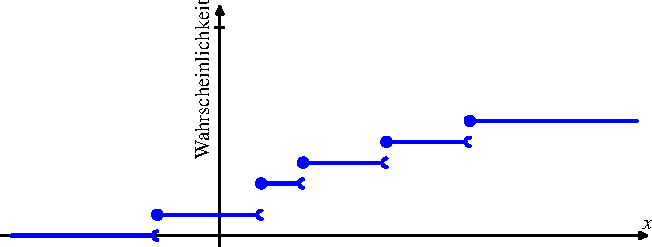
\includegraphics{images/verteilungsfunktion-3}
\[
+
\]
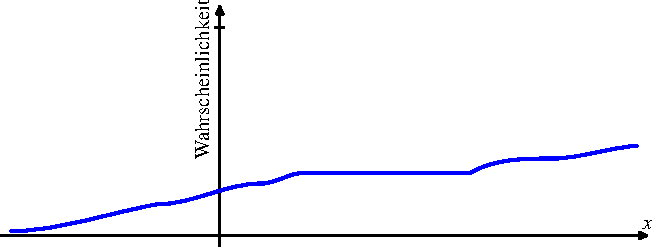
\includegraphics{images/verteilungsfunktion-4}
\[
=
\]
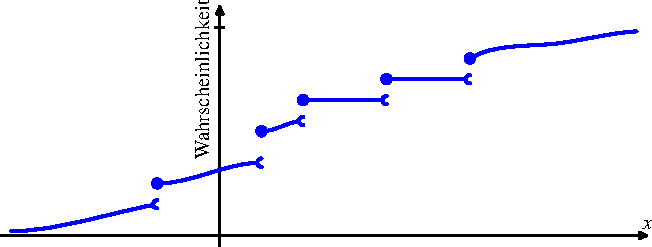
\includegraphics{images/verteilungsfunktion-2}
\end{center}
\caption{Zerlegung einer beliebigen Verteilungsfunktion (unten) in diskrete (oben)
und stetige (Mitte) Komponente\label{bildzerlegungverteilungsfunktion}}
\end{figure}
\index{Verteilung!diskrete}
\index{Verteilung!stetige}

Die Differenz $F_s=F-F_d$ kann offensichtlich keine Sprungstellen haben,
wenigstens keine Sprungstellen bei Annäherung von links.
Damit liegt
die Vermutung nahe, dass $F_s$ eine stetige Funktion ist (daher der Index
$s$).
Das ist tatsächlich so:
\begin{satz}Eine Verteilungsfunktion $F$ kann immer zerlegt werden in eine
stückweise konstante, monoton wachsende, rechtsseitig stetige Funktion
$F_d$ und eine stetige Funktion $F_s$:
\[
F=F_d+F_s,
\]
ausserdem ist diese Zerlegung eindeutig.
\end{satz}
Die Zerlegung der Verteilungsfunktion $F$ ist in
Abbildung~\ref{bildzerlegungverteilungsfunktion} dargestellt.
Der nachfolgende Beweis des Satzes ist etwas technisch, wird aber später nicht
weiter benötigt, er kann daher auch übersprungen werden.
{\small
\begin{proof}[Beweis]
Es genügt offensichtlich zu zeigen, dass $F$ rechtsseitig stetig ist, also
keine Sprungstellen bei Annäherung von rechts hat.
Die Differenz
$F(a+\varepsilon)-F(a)$ ist die Wahrscheinlichkeit, dass der Wert der
Zufallsvariable in das Intervall $(a,a+\varepsilon]$
fällt.
Es genügt, wenn man für $\varepsilon=\frac1n$ zeigen kann,
dass $F(a+\frac1n)\to F(a)$.
Das Intervall $(a,a\frac1n]$ kann man
als Vereinigung unendlich vieler kleiner Teilintervalle
schreiben, also
\[
\left(a,{\textstyle a+\frac1n}\right]
= \left(a,a+{\textstyle \frac1N}\right]\cup
\bigcup_{k=n}^{N-1}\left(a+{\textstyle\frac1{k+1}},a+{\textstyle\frac1k}\right],
\]
wobei die Teilintervalle alle disjunkt sind.
Nimmt man nun die Wahrscheinlichkeit auf beiden Seiten, folgt aus den
Axiomen für $P$
\[
P\left(\left(a,a+{\textstyle\frac1n}\right]\right)
=
P\left(\left(a,a+{\textstyle \frac1N}\right]\right)+
\sum_{k=n}^{N-1}P\left(\left(a+{\textstyle\frac1{k+1}},a+{\textstyle\frac1k}\right]\right).
\]
Der Ausdruck $P\left(\left(a,a+{\frac1N}\right]\right)$ ist also der
Rest einer unendlichen Reihe mit ausschliesslich positiven Gliedern,
mit der $P\left(\left(a,a+{\textstyle\frac1n}\right]\right)$
berechnet werden kann.
 Nach den Axiomen für $P$ gilt wegen
\[
\left(a,{\textstyle a+\frac1n}\right]
= 
\bigcup_{k=n}^{\infty}
\left(a+{\textstyle\frac1{k+1}},a+{\textstyle\frac1k}\right]
\]
auch
\[
P\left(\left(a,{\textstyle a+\frac1n}\right]\right)
= 
\sum_{k=n}^{\infty}
P\left(\left(a+{\textstyle\frac1{k+1}},a+{\textstyle\frac1k}\right]\right),
\]
d.~h.~die Reihe ist konvergent.
Also streben die einzelnen Glieder gegen null,
oder
\[
0=\lim_{n\to\infty}P\left(\left(a,{\textstyle a+\frac1n}\right]\right)
=\lim_{n\to\infty}F(a+{\textstyle\frac1n}) - F(a)=\lim_{x\to a+} F(x)-F(a),
\]
also genau die Aussage, dass die rechtsseitigen Grenzwerte mit den
Funktionswerten übereinstimmen, mithin die Funktion $F$ rechtsseitig
stetig ist.
Somit ist $F_s$ rechts- und linksseitig stetig.
\end{proof}
}
Im Allgemeinen besteht also eine Verteilungsfunktion $F$ aus einem
Teil, der Sprünge darstellt, also bestimmte Werte der Zufallsvariable,
die mit nicht verschwindender Wahrscheinlichkeit auftreten können, und
einem Teil, der ``verschmiert'' ist über den ganzen Wertebereich.
Wir
betrachten jeden dieser Teile separat.

\subsection{Stückweise konstante Verteilungsfunktion}
\begin{figure}
\begin{center}
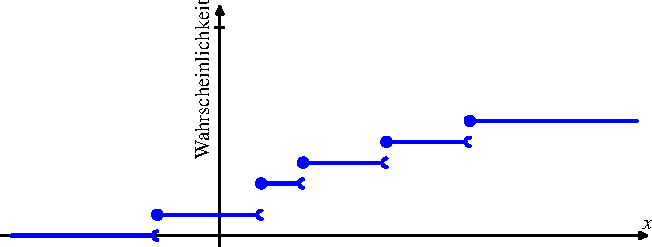
\includegraphics{images/verteilungsfunktion-3}
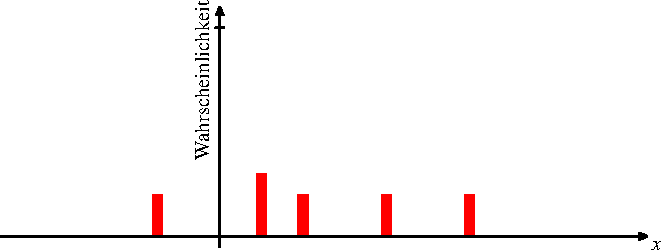
\includegraphics{images/verteilungsfunktion-5}
\end{center}
\caption{Verteilungsfunktion (oben) und Wahrscheinlichkeiten einzelner
$x$-Werte (unten) einer diskreten Verteilung
\label{bilddiskreteverteilungsfunktion}}
\end{figure}
Ist die Verteilungsfunktion stückweise konstant, dann ist
$P((a,b])=0$ falls im Intervall $(a,b]$ keine Sprungstelle
vorhanden ist.
Ist $x_0$ eine Sprungstelle, dann ist ihr Höhe
\[
\lim_{a\to x_0-}P((a,x_0])
=
\lim_{a\to x_0-}(F(x_0)-F(a))
=
F(x_0)-\lim_{a\to x_0-}F(a).
\]
Dies bedeutet, dass $P(\{x_0\})=F(x_0)-\lim_{a\to x_0-}F(a)$.
Offensichtlich haben also nur die Sprungwerte der Funktion eine
von 0 verschiedene Wahrscheinlichkeit, alle anderen Intervalle ohne
einen Sprungpunkt haben Wahrscheinlichkeit 0.
Die Wahrscheinlichkeiten
der einzelnen Sprungwerte können wie in
Abbildung~\ref{bilddiskreteverteilungsfunktion} visualisiert werden.

Ist $S=\{\,x\;|\;F(x)\ne \lim_{a\to x-}F(a)\,\}$ die Menge der Sprungpunkte 
der Verteilungsfunktion, dann kann man damit Wahrscheinlichkeiten und
Erwartungswerte wie folgt berechnen.
Die Wahrscheinlichkeit eines
Ereignisses hängt davon ab, welche Sprungpunkte es enthält:
\[
P(A)=\sum_{x\in S}P(\{x\}),
\]
der Erwartungswert von $f(X)$ ist
\[
E(f(X))=\sum_{x\in S}f(x)P(\{x\}).
\]
Man kann also alle relevanten Grössen berechnen, wenn man für jede
Sprungstelle deren Wahrscheinlichkeit weiss, also die Funktion
\[
p\colon S\to\mathbb{R}:x\mapsto p(x)=P(\{x\}).
\]
Diese Funktion muss natürlich den Eigenschaften einer
Wahrscheinlichkeitsfunktion Rechnung tragen, was erfüllt ist, wenn
$p(x)\ge 0$ für alle Sprungpunkte und 
\[
\sum_{x\in S}p(x)=1.
\]
\begin{definition}Die Funktion $p\colon S\to\mathbb{R}:x\mapsto p(x)$
heisst diskrete Wahrscheinlichkeitsverteilung auf der Menge $S$.
\end{definition}
\begin{satz}Für eine diskrete Wahrscheinlichkeitsverteilung $p$ gilt
\begin{enumerate}
\item $\displaystyle P(A)=\sum_{x\in A\cap S}p(x)$,
\item $\displaystyle E(f(X))=\sum_{x\in S}f(x)p(x)$.
\end{enumerate}
\end{satz}

\subsection{Stetige Verteilungsfunktion}
\begin{figure}
\begin{center}
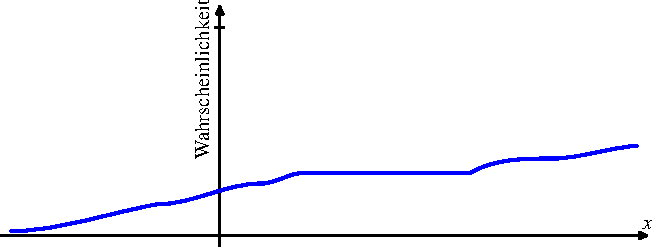
\includegraphics{images/verteilungsfunktion-4}
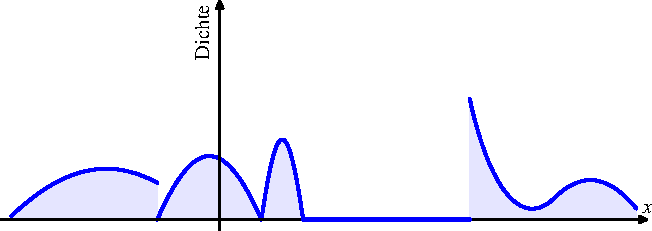
\includegraphics{images/verteilungsfunktion-6}
\end{center}
\caption{Verteilungsfunktion (oben) und Wahrscheinlichkeitsdichte 
(unten) einer stetigen Verteilung\label{bildstetigeverteilungsfunktion}}
\end{figure}
Die Formel
\[
P((a,b])=F(b)-F(a)
\]
erinnert an die Berechnung eines Integrals mit Hilfe einer
Stammfunktion.
Wäre $F$ differenzierbar, könnte man die Ableitung bilden,
$F$ wäre dann eine Stammfunktion von $\varphi=F'$.
Dann gälte
\[
P(X\le x)=F(x)=\int_{-\infty}^x\varphi(\xi)\,d\xi.
\]
Im Allgemeinen ist selbst eine stetige Verteilungsfunktion nicht
differenzierbar.
Trotzdem gibt es dank eines Satzes, den wir hier nicht beweisen,
immer eine Funktion $\varphi$, die sich ähnlich verhält wie die
Ableitung.
\begin{definition}
Die Funktion $\varphi$ heisst Wahrscheinlichkeitsdichte der Verteilungsfunktion
\index{Wahrscheinlichkeitsdichte}
\index{Dichtefunktion}
$F$ falls
\[
P(X\le x)=F(x)=\int_{-\infty}^x\varphi(\xi)\,d\xi
\]
gilt.
Man spricht in diesem Fall von einer stetigen Wahrscheinlichkeitsverteilung.
\end{definition}
Abbildung~\ref{bildstetigeverteilungsfunktion} zeigt die
Wahrscheinlichkeitsdichte der stetigen Komponente der Verteilungsfunktion
aus Abbildung \ref{bildverteilungsfunktion}.

Aus den Eigenschaften der Verteilungsfunktion $F(x)$
gemäss Definition \ref{verteilung:definition:verteilungsfunktion}
folgen sofort Eigenschaften der Wahrscheinlichkeitsdichte $\varphi(x)$.
Da $F(x)$ monoton wachsend ist, muss die Ableitung $\varphi(x)\ge 0$
sein.
Da der Grenzwert $\lim_{x\to\infty}F(x)=1$ ist, muss das Integral
über ganz $\mathbb{R}$ den Wert $1$ haben, also
\begin{equation}
\int_{-\infty}^\infty \varphi(x)\,dx = 1.
\label{verteilung:wahrscheinlichkeitsdichte:normierung}
\end{equation}
Die Gleichung \eqref{verteilung:wahrscheinlichkeitsdichte:normierung}
heisst auch die {\em Normierungsbedingung} für die Wahrscheinlichkeitsdichte.
Eine Funktion $\varphi(x)$ kann also nur die Wahrscheinlichkeitsdichte
einer stetigen Zufallsvariable sein, wenn sie nicht negativ ist und
\eqref{verteilung:wahrscheinlichkeitsdichte:normierung} gilt.

Bei diskreten Wahrscheinlichkeitsverteilungen folgte die Formel für den
Erwartungswert von $X$ sofort aus der Definition, für den stetigen
Fall haben wir aber noch keine exakte Definition.
Wenn wir $\mathbb{R}$
in viele kleine Intervalle $I_1=(\underline x_1,\overline x_1],\dots, I_n$
unterteilen, dann gilt
\[
\sum_{i}P(I_i)\underline x_i\le
E(X)
\le
\sum_{i}P(I_i)\overline x_i.
\]
Da die Wahrscheinlichkeit des Intervalls $I_i$ mit Hilfe der
Wahrscheinlichkeitsdichte berechnet werden kann:
$P(I_i)=\int_{\underline x_i}^{\overline x_i}\varphi(\xi)\,d\xi,$
kann man die Ungleichung noch etwas weiter fassen:
\[
\sum_{i}\underline x_i\bigl(\min_{\xi\in I_i}\varphi(\xi)\bigr)(\overline x_i-\underline x_i)\le
E(X)
\le
\sum_{i}\overline x_i\bigl(\max_{\xi\in I_i}\varphi(\xi)\bigr)(\overline x_i-\underline x_i).
\]
Lässt man jetzt die Intervalllänge immer kleiner werden, wird wegen der
Stetigkeit von $\varphi$ der Unterschied zwischen
$\max_{\xi\in I_i}\varphi(\xi)$ und
$\min_{\xi\in I_i}\varphi(\xi)$ beliebig klein, und auch jener
zwischen $\underline x_i$ und $\overline x_i$.
Beim Grenzübergang
zu beliebig kleinen Intervallen werden die beiden Seiten der Ungleichung
gegen das Integral
\[
\int_{-\infty}^{\infty}x\varphi(x)\,dx
\]
streben, d.~h.~der folgende Satz kann als Definition des Erwartungswertes
gesehen werden:
\begin{satz}
Ist $X$ eine Zufallsvariable mit stetiger
Wahrscheinlichkeitsverteilung mit Wahrscheinlichkeitsdichte
$\varphi$, dann
ist die Verteilungsfunktion $F$ überall dort differenzierbar, wo
$\varphi$ stetig ist, und es gilt dort
$F'(x)=\varphi(x)$.
Erwartungswerte von $X$ können mit Hilfe von
\begin{align*}
E(X)&=\int_{-\infty}^{\infty}x\varphi(x)\,dx\quad\text{und}\\
E(f(X))&=\int_{-\infty}^{\infty}f(x)\varphi(x)\,dx
\end{align*}
berechnet werden.
\end{satz}

Man beachte, dass diese Formel das im
Kapitel~\ref{chapter:erwartungswert-und-varianz} einführte Konzept
``Wert $\mathstrut \times\mathstrut $ Wahrscheinlichkeit''
auch für stetige Zufallsvariablen realisiert, $x$ bzw.~$f(x)$ ist
der Wert-Teil, während $\varphi(x)\,dx$ für die Wahrscheinlichkeit
steht.
Aus der Summe ist ein Integral geworden.

\subsection{Wahrscheinlichkeit grosser Abweichungen}
Im vorhergehenden Kapitel haben wir mit dem Satz von Tschebyscheff ein
Hilfsmittel kennengelernt, welches erlaubt abzuschätzen, dass eine
gross Abweichung vom Erwartungswert eintritt.
Der Satz stellte einen
Zusammenhang mit der Varianz her:
\[
P(|X-\mu|>\varepsilon)\le\frac{\operatorname{var}(X)}{\varepsilon^2}.
\]
Es wurde damals schon bemerkt, dass für ``weniger wilde'' Verteilung mit
besseren Abschätzungen gerechnet werden kann.
Insbesondere ist es mit
einer Dichtefunktion möglich, die Wahrscheinlichkeit einer grossen
Abweichung exakt zu berechnen:
\begin{satz} Ist $X$ eine Zufallsvariable, deren Verteilung die
Verteilungsfunktion $F$ hat, dann ist
\[
P(|X-\mu|>\varepsilon)=
1-F(\mu+\varepsilon)+\lim_{\xi\to (\mu-\varepsilon)-}F(\xi).
\]
Ist $\varphi$ eine Dichtefunktion, dann gilt
\[
P(|X-\mu|>\varepsilon)=1-\int_{\mu-\varepsilon}^{\mu+\varepsilon}\varphi(x)\,dx.
\]
\end{satz}
\begin{proof}[Beweis]Die Formel für die Dichtefunktion folgt offensichtlich
aus der Aussage über die Verteilungsfunktion, denn dann ist $F$ stetig
und der einseitige Grenzwert ist gerade der Funktionswert von $F$ an der
Stelle.
Es genügt also letzteres
zu untersuchen.
\begin{align*}
P(|X-\mu|\le\varepsilon)
&=1-P(\{X\ge\mu-\varepsilon\}\cap\{X\le\mu+\varepsilon\})\\
&=1-F(\mu+\varepsilon)+\lim_{\xi\to (\mu-\varepsilon)-}F(\xi).
\qedhere
\end{align*}
\end{proof}
Eine Wahrscheinlichkeitsfunktion erlaubt also eine wesentlich
genauere Berechnung der Wahrscheinlichkeit einer grossen Abweichung,
nicht mehr nur eine grobe Abschätzung.

